\newcommand{\mercenaryDescription}{
\section{Mercenary}
%\epigraph{\textit{
%    "Mercenary quote"
%} }{
%    Mercenary quotee
%}
%    Some Description
%    \\
    See \nref{tlttree:mercenary} for more information.
}

\newcommand{\mercenaryTree}{
    \newpage
    \subsection{Mercenary Talent Tree}
    \label{tlttree:mercenary}

    \textbf{Class Skills:} Brawl, Coercion, Discipline, Leadership, Melee (Heavy), Melee (Light)
    \newline

    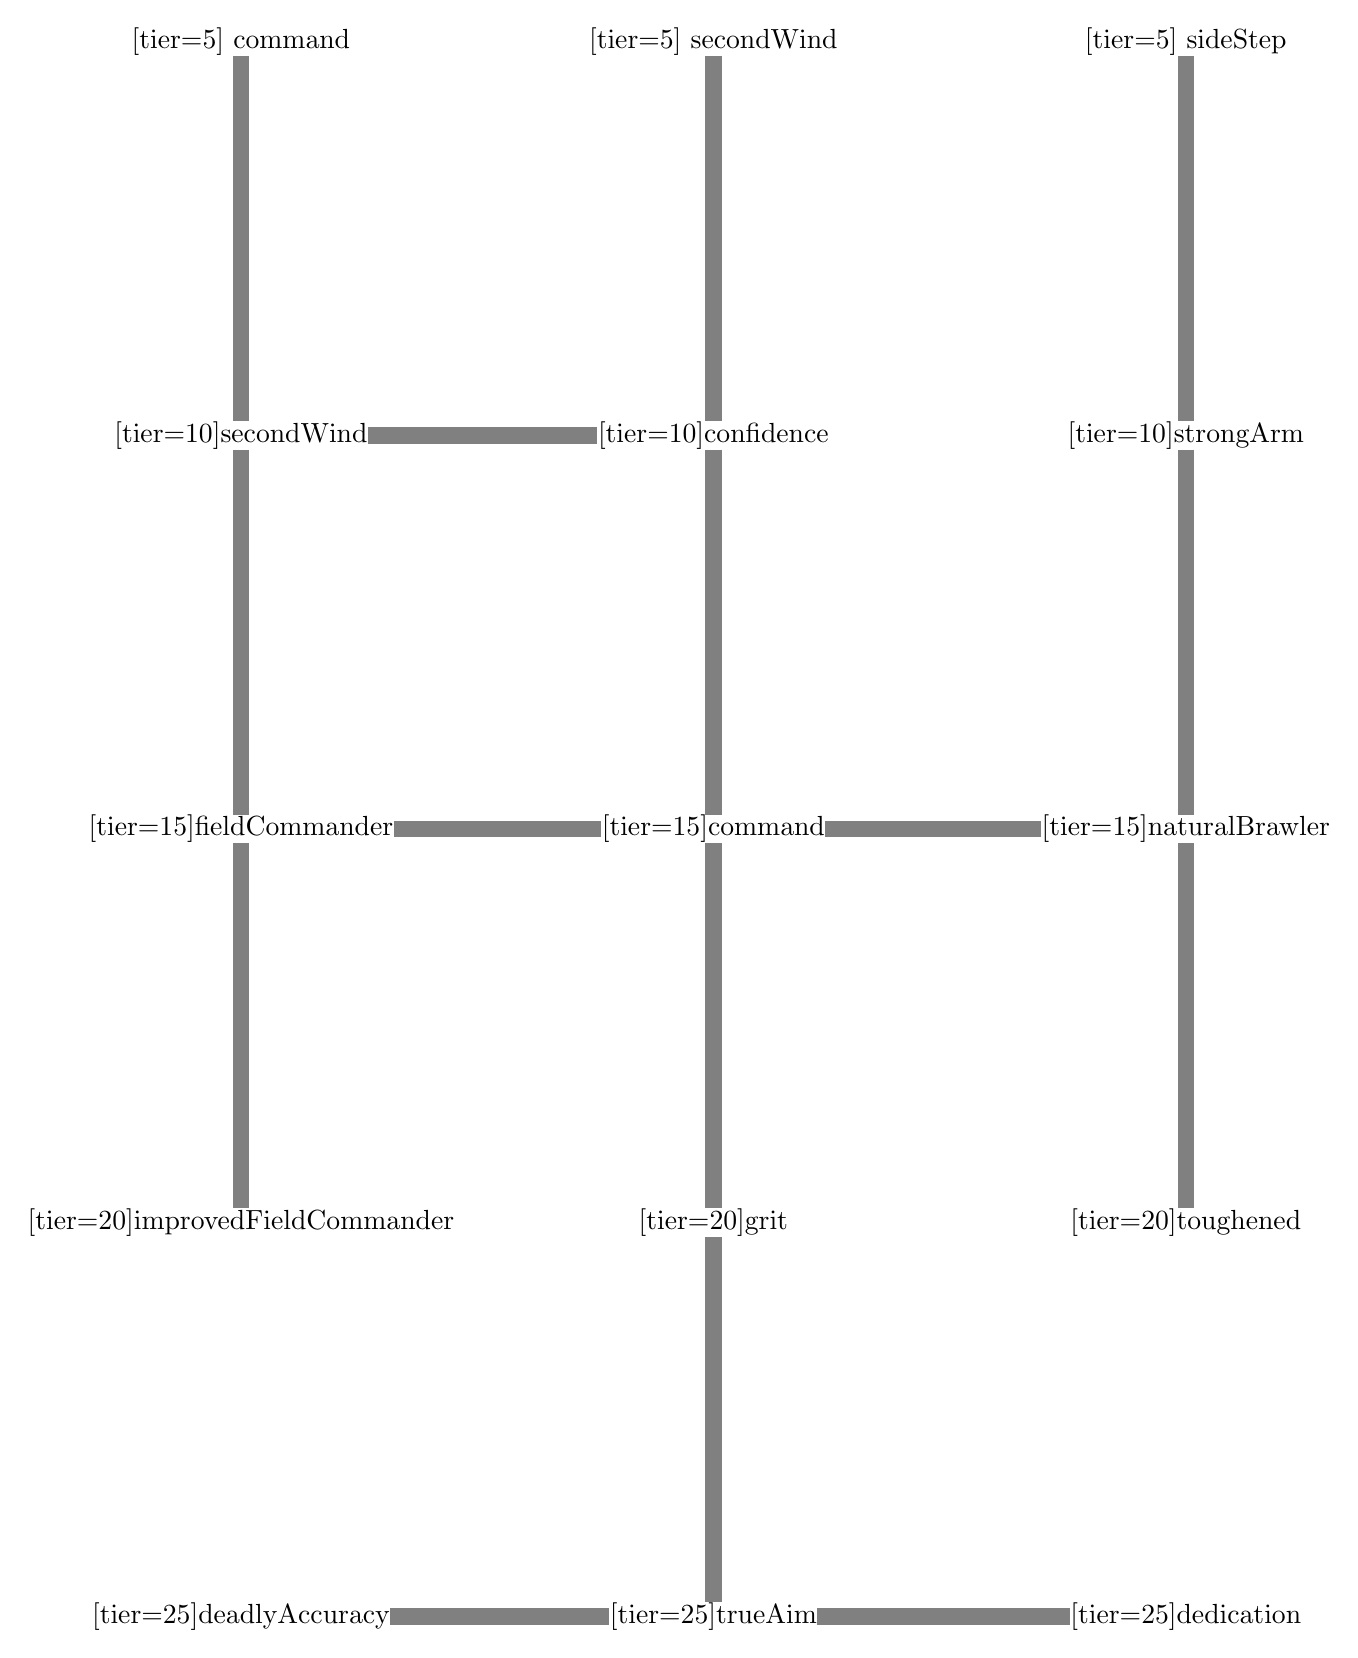
\begin{tikzpicture}
        \draw ( 0,  0) node(aa)[inner sep=0]{\TalentBox[tier=5] {command}}
              ( 6,  0) node(ab)[inner sep=0]{\TalentBox[tier=5] {secondWind}}
              (12,  0) node(ac)[inner sep=0]{\TalentBox[tier=5] {sideStep}}
              ( 0, -5) node(ba)[inner sep=0]{\TalentBox[tier=10]{secondWind}}
              ( 6, -5) node(bb)[inner sep=0]{\TalentBox[tier=10]{confidence}}
              (12, -5) node(bc)[inner sep=0]{\TalentBox[tier=10]{strongArm}}
              ( 0,-10) node(ca)[inner sep=0]{\TalentBox[tier=15]{fieldCommander}}
              ( 6,-10) node(cb)[inner sep=0]{\TalentBox[tier=15]{command}}
              (12,-10) node(cc)[inner sep=0]{\TalentBox[tier=15]{naturalBrawler}}
              ( 0,-15) node(da)[inner sep=0]{\TalentBox[tier=20]{improvedFieldCommander}}
              ( 6,-15) node(db)[inner sep=0]{\TalentBox[tier=20]{grit}}
              (12,-15) node(dc)[inner sep=0]{\TalentBox[tier=20]{toughened}}
              ( 0,-20) node(ea)[inner sep=0]{\TalentBox[tier=25]{deadlyAccuracy}}
              ( 6,-20) node(eb)[inner sep=0]{\TalentBox[tier=25]{trueAim}}
              (12,-20) node(ec)[inner sep=0]{\TalentBox[tier=25]{dedication}}
        ;

        \tikzstyle{bar}=[gray,-,>=stealth, line width=6pt]

        \draw [bar] (aa) to (ba);
        \draw [bar] (ab) to (bb);
        \draw [bar] (ac) to (bc);

        \draw [bar] (ba) to (ca);
        \draw [bar] (bb) to (cb);
        \draw [bar] (bc) to (cc);

        \draw [bar] (ca) to (da);
        \draw [bar] (cb) to (db);
        \draw [bar] (cc) to (dc);

        \draw [bar] (db) to (eb);

        \draw [bar] (ba) to (bb);

        \draw [bar] (ca) to (cb);
        \draw [bar] (cc) to (cb);

        \draw [bar] (ea) to (eb);
        \draw [bar] (ec) to (eb);
    \end{tikzpicture}
}
